\chapter{Discussion}\label{ch:disc}

Up to now this research is presented first by describing the model, followed by the presentation of a series of experiments. The model is built such that the robots can engage in language games, for which the physical interactions have been pre-programmed. The language games consists roughly in four parts: (1) the robots detect their surroundings, (2) the sensing is categorised, (3) the speaker names one topic and the hearer tries to understand the speaker's utterance, and (4) the robots adapt their ontologies and lexicon.

An important feature of the experiment is that the robots do not have any prior knowledge about the ontology or lexicon. They only have knowledge how they can communicate and how they can invent, adopt and select ontological and lexical items that enables them to develop a coherent communication system. 

The main questions raised in the introduction of this book were:

\begin{enumerate}
\index{symbol grounding problem}
\item Can the symbol grounding problem be solved with these robots by constructing a lexicon through individual adaptation, (cultural) interaction and self-organisation? And if so, how is this accomplished?
\index{extra-linguistic information}
\item What are the important types of extra-linguistic information that agents should share when developing a coherent communication system?
\item What is the influence of the physical conditions and interaction on developing a grounded lexicon?
\end{enumerate}

Question (1) can reasonably be answered with {\em yes}, at least within the current application and experimental set-up. There are some drawbacks on this answer, because some important assumptions have been made and the physical capabilities of the robots prevent to enable perfect sensing and communication. The two assumptions were that the robots could establish joint attention and provide feedback on the outcome of a language game. Previous experiments on physical pointing revealed that this method does not work with the currently used robots \citep{vogt:1998b}, and hence the robots still need to have a way in doing so. In the experiments the robots were able to inspect each other's internal feature vectors. This way the robots were able to construct a shared and grounded lexicon. The symbol grounding problem has been solved in the experiments reported by a number of subtasks as will be discussed in the next section.

The answer to question (2) is not complete, because not all possible forms of information have been investigated. Nevertheless, some important forms have been found. It appeared that establishing joint attention is very important in the development of a coherent lexicon. When joint attention is not established, feedback plays a crucial role.

The last question is harder to answer, because not all experiments yielded astonishing results. However, there are some important conclusions that can be drawn. The sensing and segmentation, resulted in set of situations in which approximately 20 \% did not have a coherent context. So only 80 \% of the language games the robots could establish communicative success, because in the other cases the hearer did not detect the topic that the speaker was communicating. The impact from varying physical conditions has not been shown convincingly in all proposed directions. Although, they indicated some influences.


This chapter will discuss the results in more detail, and will compare the findings with the literature. Section \ref{s:disc:global} will discuss how the grounding problem is solved. The effect of joint attention and feedback will be the topic of \sectref{s:disc:feed}. The experimental results will be discussed around psychological issues about joint attention and feedback in language learning. The influence of the physical interactions will be discussed in \sectref{s:disc:phys}. Especially the robots' adaptation to the environment (or vice versa) is the key issue. In \sectref{s:disc:th} the results will be compared with other experiments on grounding language, especially the Talking Heads \citep{belpaeme:1998} and the work of \citet{billard:1997a}.

\section{The Symbol Grounding Problem Solved?}\label{s:disc:global}
\index{symbol grounding problem}

The key problem that had to be solved for physical robots to develop a shared lexicon about the things they detect is the symbol grounding problem \citep{harnad:1990}. The problem is how seemingly meaningless symbols can become meaningful in the real world. In \chapref{ch:intro} three sub-problems of the grounding problem have been identified from \citep{harnad:1990}. These sub-problems are:

\begin{enumerate}
\item Iconisation\index{symbol grounding problem!iconisation}
\item Discrimination\index{symbol grounding problem!discrimination}
\item Identification\index{symbol grounding problem!identification}
\end{enumerate}

The three sub-problems will be discussed in more detail below. Solving the symbol grounding problem is known under the roboticists as a fundamentally hard problem, see e.g. \citep{pfeiferscheier:1999}. It is especially hard, because the robots have different sensings of some real world object when detected under different circumstances. It appears to be very hard to acquire invariant categorisations of these different sensings.

The symbol grounding problem has been attacked with a semiotic view towards symbols (or signs). In this Peircean view a symbol is a semiotic sign where its form is either arbitrary or conventionalised. The sign is a triangle of which the edges resemble a referent, a meaning and a form. It has been argued that a robot can ground a symbol when a semiotic triangle can be constructed successfully. Its success is measured with the success of a language game, but it can also be measured otherwise. When the symbol is used successfully in a language game, the form is said to be conventionalised.


In the experiments the real world consists of light sources about which the robots try to {\em construct} a lexicon. The word-forms and referents are the overt part of the symbols that the robots ground. The covert part is a hybrid chain of internal and possibly external structures from which the meaning is constructed. Part of these structures are activated by the robot's sensing. The sensing is segmented and feature vectors are extracted. These feature vectors are then categorised. The robots were able to successfully incorporate the distinctive categories that constitute the meaning in language use (i.e. in naming the referents). It should be clear that when the robots communicate successfully, the utterance refer to one of the light sources their environment. Whether or not this justifies to conclude that the robots have meaning in the philosophical sense where meaning is often ascribed in terms of intentionality and consciousness remains a philosophical question. Technically, the robots closed the semiotic triangle (or square) and conventionalised the form. Hence the physical symbol grounding problem is solved by these robots.


\subsection{Iconisation}\index{symbol grounding problem!iconisation|(}

Iconisation is the first step in solving the symbol grounding problem. It is related to the following question: How does the analogue sensation of a referent project on an internal representation of the robot? This representation is still sub-symbolic. Iconisation is solved in the presented application through sensing, segmentation and feature extraction. Segmentation of the raw sensory stimuli results in a set of segments that are supposed to relate to sensed real world objects. The segments consist of for noise filtered raw sensory data. Feature extraction result in a vector of features that describes each segment with invariant properties of the sensing of a real world object. This latter process is very crucial for the result of the grounding problem. Although this issue has not been a key issue in this dissertation, the problems became clear during the development of the system. 

\index{segmentation}\index{sensing}
First of all, the segmentation process has to identify those regions that are interesting and should relate to the sensing of a referent. Ideally, segmentation should identify each referent that could be detected. The robots move around in their environment and the lighting conditions may change or something can obscure (a part of) the environment. Therefore, the sensing of the different robots are not likely to be identical and neither are the different sensings in different situations. A rather simplistic segmentation scheme has been used, which is prone to errors. 

Segments are identified when the sensor value of a certain sensor exceeds a pre-determined noise value. But when, for instance, two light sources are detected shortly after each other with the consequence that one or more sensors did not get back to drop below the noise value, the two light sources will be taken as one segment. This is one of the reasons why the robots do not establish a coherent context. ``Why not identify only the top of the peaks? This way you solve this problem.'' is an often heard remark. However, the sensors are not extremely reliable and show fluctuations during the sensing of a region of interest, resulting in local maxima when looking for real maxima. Thus yielding the same problem of context incoherence. One region of interest may be segmented in several regions, making it hard to solve discrimination and identification. Increasing the noise level would cause the robots to miss light sources that are further away.

\index{feature!extraction}
When a segment is found the sensory data of such a segment is transformed into a multidimensional feature vector, where each dimension corresponds to one sensory channel. This is done by means of feature extraction. The feature extraction is done by a real valued function from the sensory channel space to the feature space. The feature space is typically taken as a real valued domain between 0 and 1 in all dimensions. The goal of this feature extraction is (1) to reduce the amount of sensory data and (2) to extract information that is ideally invariant in the different situations.\index{invariance} In the current implementation, all maxima that are found for the different sensory channels inside a segment are normalised to the maximum intensity of the sensory channel that has the highest maximum intensity in this segment. The absolute maximum of a sensory channel in a segment tells the observer to which light source the segment corresponds. Applying the feature extraction to this sensory channel results in a feature with a value of 1. Application to the other sensory channels yield values lower than 1. After feature extraction, the segment can be described with a low dimensional vector with a value of 1 where the sensory channel has the highest intensity. The other features have, depending on the distance of the robot to the corresponding light source, a value between 0 and 1. This is most often close to 0. 

So, the segmentation and feature extraction is an important pre-process in the process of solving the grounding problem. This is a widely accepted phenomenon that is applied both in (computer) vision \citep{cotter:1990} and speech perception \citep{damper:2000}. Cotter notices the fact that in a survey amongst different animal species, the optic pathways where the initial filtering takes place differ in details,  although there are fundamental similarities:

\begin{quote}
Such differences-differences in size of the pathways and development in nuclei in visual centres-represent variations on a theme that are due to the evolution of the visual system, the accentuation of specific sensory systems and ultimately the attainment of a specific ecological niche by individual species. \citep[11]{cotter:1990}
\end{quote}

This makes it plausible that pre-processing of visual stimuli is very important for categorisation. Furthermore, it sheds light on the nature of embodiment. Different ways of sensing yield different categorisations. Obviously, the feature extraction functions could be evolved  genetically as is shown in \citep{belpaeme:1999}, and once primitive functions are present, the feature extraction functions could also be developed onto-genetically into more complex ones as shown by \citet{dejong:1999}. 


Although its importance, the segmentation and feature extraction is not a key issue of this book. The segmentation and sensory channels are relatively simple and not very well developed. 
\index{symbol grounding problem!iconisation|)}

\subsection{Discrimination}\index{symbol grounding problem!discrimination|(}

The second part of the solution of the grounding problem is discrimination. Harnad (1990) applies the notion of discrimination to the level of sensing. According to Harnad, discrimination should find out how the perception of something differs from the perception of something else. This can already be done at the perceptual level. This perceptual level can be compared to the sensing, segmentation and feature extraction in the current application. Although some of the discrimination is already done with segmentation and feature extraction, it is mainly pursued at the categorisation level. Segmentation yields the different sensings of the different referents. The feature extraction describes what properties the different segments have. However, it is only at the categorisation level that the model proposed tells the robots how the different segments differ.

In the current book, discrimination is solved by modelling {\em discrimination games} \citep{steels:1996b}. In a discrimination game, an individual robot categorises the feature vectors that relate to the segments. Then the agents select categories that can distinguish a segment from the other segments in the context. So, the resulting distinctive categories only are distinctive in contrast to the context. This is conform a pragmatic approach. As a consequence, part of the meaning is in the robot's environment, making it a situated approach \citep{clancey:1997}. Since the meaning is constructed based on the robot's experience, it is embodied \citep{lakoff:1987}. This dialectic approach favours what Jordan \citet{zlatev:1997} called situated embodiment. It is also an argument for talking about the {\em physical symbol grounding problem} rather than the physical grounding problem \citep{brooks:1990} or the symbol grounding problem \citep{harnad:1990}.


So, discrimination already starts at the segmentation level. At this level the different interesting regions are identified, thus distinguishing one region from another. However, this does not answer the question how one segment is different from another. This can be answered more constructively at the categorisation level.

\index{discrimination game}
The first step of the discrimination game is categorising the feature vectors of the segments. The main method that has been used was the prototype method. Here the categories are represented by prototypes, and the feature vectors are categorised with those prototypes that are nearest to the feature vectors in the different feature spaces. The categories are organised in different feature spaces to allow categories that resemble more generalised and specialised samples of a feature vector.\index{categorisation}

The second step in the discrimination game is to extract the categories that distinguish one segment from the other segments in the context that a robot has constructed in a language game. This phase is the actual {\em discrimination}.\index{discrimination}

Initially, there are no categories at all. When the discrimination fails, new categories are created for which the features of a feature vector acts as exemplars. These prototypical categories are organised hierarchically in the different versions of the feature space. Each version of the feature space has a different resolution, thus allowing generality and specificity of the categories. In \citep{dejongvogt:1998} no such hierarchical layering was imposed and the robots had great difficulty in developing a coherent communication system. \index{prototype}\index{category!prototypical}


The categories have been made dynamic in the sense that the prototypes move in the feature space and thus their sensitivity range changes in time. It is thought that this would let the prototypical categories evolve towards a more representative sample of the feature vectors that have been extracted. In turn, this is supposed to increase the quality of the categorisation and discrimination. The experiment where this dynamical mechanism has been left out showed that this does not necessarily contributes to a higher performance. This, however, may be due to the simplicity of the robots' visual environment. Perhaps in a more complex environment it may well be very beneficial to have dynamically changing categories.

The feature vectors that the robots extract from the segments are categorised in each feature space with that category that is nearest to the feature vector. The prototypes of a feature space cover the entire space. This has the advantage that whenever there is a category in some feature space the feature vector will be categorised. When the categories are constructed with the binary subspace method, or in the binary tree method \citep{steels:1996b} as is the case in the Talking Heads, a category is only activated when the feature vector to be categorised falls inside the sensitive region of a category. This is because these categories do not necessarily cover the entire feature space. Furthermore, the binary category, once established, is not dynamic, i.e. its sensitivity does not move. Whether these are problems is not really shown. The fact that in the prototype method explored here, the robots can exploit more categories in the discrimination games increases the chance of success. This is probably the main reason why this system outperforms the experiment incorporating the binary subspace method.

Although it might be beneficial allowing fuzzy\index{category!fuzzy} boundaries on the categories' sensitivity, this has not been observed in the experiment which investigated this. No big and significant differences have been observed, except in the discrimination success, which was slightly lower. The reason for this can be found in the fact that in the fuzzy approach a feature vector can be categorised in more ways than in the non-fuzzy prototype method. This increases the probability that more feature vectors share the same categories. Hence discrimination would be more difficult. Applying the fuzzy boundaries in more complex environments, might still be beneficial, but the problem in applicability lies in the increase of computational power.


The discrimination works well. In the basic experiment the discrimination success was already approximately 92 \%.\index{discriminative success} It has been argued in \chapref{ch:basic} that the discrimination success did not go to a 100 \% because: (1) A success-rate of 100 \% simply cannot be reached. (2) The discrimination success is partly a function of the number of language games and the hearer does not play a discrimination game every language game. When the speaker did not utter a word-form or when the hearer does not know the word-form no discrimination game is played. These reasons are confirmed with the results of letting the agents only playing discrimination games. It appeared now that the average discrimination success rose to 98.7 \%.

The meanings that emerge are used very distinctive. In all experiments the distinctiveness\index{distinctiveness} is higher than 0.95 and usually ends up with a value of 1. So, when a distinctive category is used in the communication it refers to the same referent with a high certainty. It is well shown in the meaning-referent competition diagrams that after a very short period, the meanings that are used in the language refer to the same referents about 100 \% of the time. The parsimony\index{parsimony}, however is lower. The probability that when trying to categorise a referent with a previously used category is around 0.85. It can be explained by the fact that in different situations the segments differ and hence are categorised differently, thus yielding a strong one-to-many relationship between a referent and the distinctive categories.

In these experiments, the categories all bear the invariant property that the dimension of the feature vector with value of 1 corresponds to a unique referent. In the Talking Heads invariance is filtered out using the notion of saliency.\index{saliency} However, as the statistics of the sensory data revealed (appendix C), saliency does not guarantee to find the invariance. This is because another dimension of the feature vector might have a value very close to 1, which may not be most salient. However, there may be selection criteria in the discrimination or naming game that allows a more controlled categorisation of invariant properties of the different feature vectors. A possible mechanism preference could be the selection of categories that have maximum values at their sensory channels. However, this would require to implement more knowledge on the categorisation, which is against the non-nativist approach that is pursued. On the other hand, selection for maximum intensity is so simple and uniform that such a selection principle could have evolved genetically. Still another selection criterion may be how well a feature vector correlates with a prototype. I.e. an agent may prefer those categories of which the extracted feature values best resemble the categories. This way a prototype effect \citep{rosch:1976} could be modelled.\index{prototype!effect}\index{Rosch, Eleanor} Naturally, these different criteria could be combined yielding a hybrid mechanism.  \index{category!prototypical}


According to \citet{harnad:1990}, one of the aims of discrimination is to reduce the amount of symbolic structures that relates to a certain referent. As \figref{f:opt:words} showed, the number of distinctive categories that have been proposed can increase up to more than 2,500 for categorising 4 referents! Although it has not been shown in this book, it has been observed that when counting all different (non distinctive) categories that has been proposed before discrimination was applied, more than 5,000 (sometimes even 10,000) categories were constructed. So, the discrimination already yields a substantial reduction in the amount of categories that relate to the different segments. The naming phase further reduces the number of categories to, say 500 meanings that are used successfully in the communication. Of these 500 meanings, most are rarely used, while a few are used most frequently as observed in the various competition diagrams. It should be clear that  discrimination games alone cannot solve the grounding problem sufficiently. Still too many distinctive categories are categories for the four referents.
\index{symbol grounding problem!discrimination|)}

\subsection{Identification}\index{symbol grounding problem!identification|(}

A final process in symbol grounding is identification. Identification is reducing the symbolic structures relating to a segment even more than is the case in discrimination yielding invariant symbols.\index{invariance}\index{symbol} As argued before, the identification process of symbol grounding takes place at the language level. In other applications or types of problem solving, identification may take place at a different level depending on the type of problem to be solved. For planning a path, for instance, a robot also has to identify symbols with which it can reason. Then identification succeeds when the robot successfully incorporates the symbols to plan a path. In language this is at the communication level. When a language game is unsuccessful, at least one of the robots failed to identify the referent and it is not sure which robot failed to do so. Therefore, identification is successful when the language game is a success.\index{referent}

It is at the identification level that a distinctive category becomes a meaning. As argued, a meaning is some categorisation that is used in language. It is a part of the symbol that has been defined in semiotics. There the meaning is the {\em sense} that is made of the symbol. According to \citet{wittgenstein:1958} the meaning can only be interpreted by its use in language. Therefore, it should be related with a form that can be used in a language game. This trinity (referent, meaning and form) is what Peirce called a symbol. \index{referent}\index{form}\index{meaning}\index{symbol}\index{semiotics}\index{Wittgenstein, Ludwig}\index{Peirce, C.S.}

The basic experiment\index{basic experiment} already showed that the robots solved the grounding problem in successful language games. They successfully identified symbols that stand for a referent. However, there was still quite some polysemy. Although higher than the a priori success, the communicative success-rate\index{communicative success} was relative low. In chapters \ref{ch:lex} and \ref{ch:opt} it has been shown that the success could increase and thus identification improved. The main factors that improved the success were: assuming joint attention, increasing the form creation rate and learning rate, and assuming a different form-adoption scheme.

The influence of the form creation probability ($P_s$) has been shown in \sectref{s:par:ps}. It appeared that increasing the creation probability increased the success in communication. It also increased the specificity, i.e. the likelihood that when a word-form is used it would refer to the same referent it previously referred to increased. Increasing the creation probability, however revealed a major drawback: the number of word-forms used increased proportionally up to 83 when $P_s=1.0$. This sums up to more than 20 word-forms per referent, which is not very efficient. The point is that a high creation probability decreases the amount of many-to-many relations between meaning and form, which in turn increases the specificity\index{specificity} because the meanings uniquely refer to a particular referent. This is nice, but it increases synonymy. The number of word-forms used are much lower when $P_s=0.1$ and the communicative success is not much lower than when $P_s=1.0$ (only a few percent, but significantly). Now only 25 word-forms are used, yielding slightly more than 6 word-forms per referent. \index{form!creation probability}

When, in addition, the hearer is allowed to adopt the speaker's word-form\index{form!adoption} when it misinterpreted the speaker's utterance, the success grows even more and the number of word-forms used decrease even more. In the optimal guessing game experiment ($P_s=0.1$), where also the learning rate is different from the basic experiment, the number of word-forms used are 16, most of them used rarely. Inspecting the experiment more closely, there are only 6 word-forms that are used frequently. The communicative success grows up to approximately 75 \% after 10,000 language games. So, it seems that adopting the word-forms after misinterpretation is one of the necessary factors of the model. Furthermore, in less reliable robots, a modest creation probability is very useful: It allows the word-forms to be associated with more meanings, thus increasing the amount of one-to-many relations between form and meaning. The adaptation of the association scores\index{score!association} and lateral inhibition\index{lateral inhibition} causes improved selection and through self-organisation\index{self-organisation} a more coherent and invariant lexicon emerges.\index{invariance} This way referential polysemy and synonymy remain low.\index{polysemy}\index{synonymy}

A high learning rate, controlling the adaptation of the association scores, increases the influence of past success and has low influence on failures. When the learning rate\index{learning rate} is too high ($\eta=0.99$), the system does not find a suitable equilibrium in the scores. Failures are not punished and will be made again, thus the success does not increase. Lateral inhibition is small and the lexicon does not converge well enough to an attractor. A suitable lexicon also does not emerge when the learning rate is too low, i.e. when $\eta \leq 0.1$. If there is no word-form adoption when the hearer misinterpreted the speaker, the self-organising effect that the score adaptation should control does not reveal itself.


So, identification in the language games takes place at the language level. The invariance of the symbols are therefore to be found in the consistent use of these symbols in the language. This way the ambiguous categorisation of the various sensings of some referent is disambiguated in the successful use of the symbols in the language games.
\index{symbol grounding problem!identification|)}

\subsection{Conclusions}

\begin{figure}
\centerline{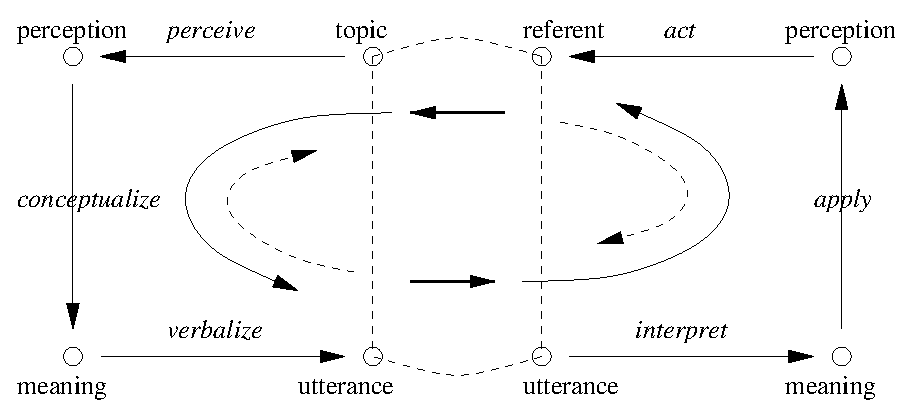
\includegraphics[width=12cm]{discr_games/semiotic1.eps}}
\caption{The semiotic square of the language games.\index{semiotic landscape}}
\label{f:disc:semiotic}
\end{figure}

The hybrid processes of sensing, segmentation, feature extraction, categorisation, discrimination, naming and feedback transforms the symbol grounding in the formation of a semiotic coupling (or structural coupling) \index{structural coupling} between the robots' environment, their internal states and their mutual interaction. Some of the lexicons that result from the experiments have been plotted in semiotic landscapes\index{semiotic landscape} showing the structural couplings that emerged. These landscapes showed that the many-to-many relations between form and meaning can serve cognitive agents to decrease the amount of polysemy and synonymy that is necessary to ground their sensing of the environment invariantly.\index{invariance}

The meaning of the utterances are always in contrast to the rest of the context as a result of the discrimination game. However, the experiment with only three of the four light sources present in every situation showed that the robots acquired a lexicon similarly to the basic experiment. Hence the system learns to communicate about the four referents in their world, while only sensing three in their environment. Nevertheless, the use of the language depends on the situation that the agents are in.

So, the symbol grounding problem is solved by a hybrid of relative simple mechanisms: sensing, segmentation, feature extraction, categorisation, discrimination, naming and feedback. The principles are based on interactions of the agents with their environment and each other, individual adaptation and self-organisation. A complex structure of couplings emerges from the co-evolution of language and meaning,\index{co-evolution} and can well be used to communicate about the agents' environment. Summarising, the three phases of the symbol grounding problem are modelled by the following:

\begin{enumerate}
\item {\bf Iconisation:} Sensing, segmentation and feature extraction.
\item {\bf Discrimination:} Discrimination game.
\item {\bf Identification:} Naming and adaptation.
\end{enumerate}

One of the main findings was that the robots tend to categorise the various sensings of a particular referent differently. Thus yielding one-to-many relations between referent and meaning. This is not problematic as long as this is cancelled out by one-to-many relations between form and meaning. This results in low, or ideally no polysemy and synonymy as illustrated in \figref{f:disc:semiotic1} (a). The proposed model is pretty well capable of doing just this. Figure \ref{f:disc:semiotic1} shows how a symbol thus can be visualised by a set of semiotic triangles. These types of symbolic structures may well explain the notions of family resemblance (fig. \ref{f:disc:semiotic1} (b)) and object constancy (fig. \ref{f:disc:semiotic1} (c)).

\begin{figure}
\centering
\subfigure[]{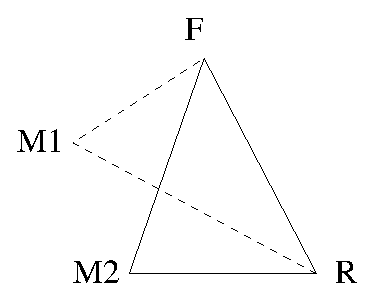
\includegraphics[width=5cm]{Discussion/sem1.eps}}
\subfigure[]{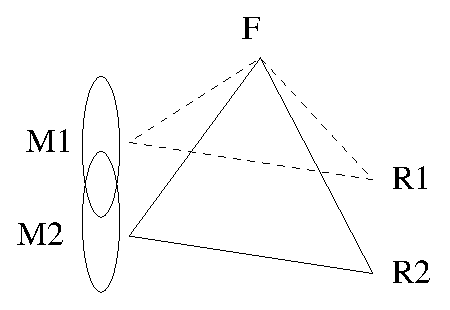
\includegraphics[width=5cm]{Discussion/famres.eps}}\\
\subfigure[]{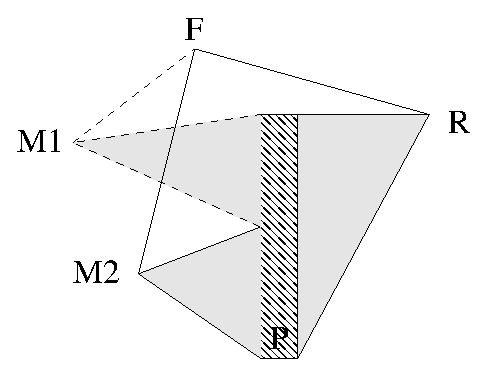
\includegraphics[width=6cm]{Discussion/objcons.eps}}
\caption{Illustration of three semiotic relations between referent R, meaning M and form F. Figure (a) shows how one-to-many relations between referent and meaning cancels out synonymy and polysemy by one-to-many relations between form and meaning. Figure (b) shows how the model may explain family resemblance. The ovals should be interpreted as venn-diagrams of the meanings M1 and M2. In figure (c) the continuum of possible sensings P of referent R are displayed as a rectangle. Some part of the rectangle may be interpreted by M1 and another by M2. When both meanings relate to the same form, this mechanism may solve the problem of object constancy.}
\label{f:disc:semiotic1}
\end{figure}


\index{family resemblance} Family resemblance \citep{wittgenstein:1958} is the observation that seemingly different things are called the same without being ambiguous, like the meaning of {\em games}. Where soccer and chess are typical games, a game like swinging is not typical. Swinging lies near the border of the 'conceptual space' of games. It has no direct resemblance with games like soccer  and chess (referents R1 and R2 fig. \ref{f:disc:semiotic1} (b)), but it has some resemblance with other games that in turn do have resemblance with soccer and chess. Such categorisation process can be explained with the one-to-many relations between form and meaning. The word {\bf games} is associated with different meanings of soccer, chess and swinging. The successful use of these meanings in different situated language games allows the system to emerge a family of resemblance.


One of the reasons that makes the symbol grounding problem hard is the notion of object constancy. How can an object be recognised as being the same when different sensings of such an object results in different sensory stimuli, for instance because it is partly obscured? In the experiments, the robots detect the light sources from different positions, resulting in different sensings as the continuum of sensings P in \figref{f:disc:semiotic1} (c) shows. This may also yield different meanings. Nevertheless, the system identifies the objects pretty consistently, because the one-to-many relations between form and meaning is damped at the level of form and referent. That the robots actually learn to identify the referents has been shown in an experiment where there were only three of the four referents available in each situation. The robots could learn to name all referents equally well as in the basic experiment whereas they only could detect three of them in a situation.\index{object constancy}


\index{symbol grounding problem|)}

\section{No Negative Feedback Evidence?}\label{s:disc:feed}
\index{feedback|(}
\index{no negative feedback evidence|(}

The experiments in \chapref{ch:lex} showed the importance of either joint attention or feedback in the language formation. One experiment has been done in which neither are present: the XSL game. In this experiment the robots used association scores based on the co-occurrences of word-meaning associations to select them. A XSL game was considered to be successful when the hearer 'thought' it understood the speaker. The communicative success\index{communicative success} from the robots' viewpoint was around 82 \%, but the actual success\index{actual success} was in fact less than 25 \%, which is lower than the a priori success. 

\index{language!acquisition}

Many psycholinguists hold that children when learning language hardly get any feedback on their language use. This is the so-called {\em no negative feedback evidence}, see e.g. \citep{braine:1971,bowerman:1988}\footnote{Recall that feedback in this book is about the effect of a language game; not to correct one another.}. Other psycholinguist claim that when children make (structurally the same) mistakes, they do get feedback from their language teachers like their parents \citep{demetrasetal:1986}. Furthermore, the influence of feedback on language acquisition is thought to be crucial by some scientist \citep{clancey:1997,demetrasetal:1986,clarkclark:1977,tomasellobarton:1994}. The results of the guessing game and the XSL game make clear that this model seems to be unable to work without feedback. The fact that when the robots mismatch in referent word-form adoption\index{form!adoption} benefits the communicative success provides a strong reason why feedback is needed in the guessing game. 

Although less successful in communication than the observational game, or perhaps only slower, the guessing game appears to converge best on the lexicon. Mostly, a clear winning name is used by the robots and the competition at the bottom is not successful. Since the hearer has no knowledge about the topic prior to linguistic communication, it has to trust completely on the linguistic information. The robots have to disambiguate the lexicon for which feedback is required. When the feedback only depends on the co-occurrence of word and meaning as is the case in the XSL game, the robots cannot disambiguate the system well. The feedback must be on the success of the language game. Since communication in the guessing game is not redundant as in the ostensive and observational games, there is more pressure to disambiguate. Hence the robots are better at it.



When joint attention is established prior to the communication, directive feedback appears to be less important. \index{joint attention}Experiments revealed that when the robots established prior topic knowledge (or joint attention prior to the communication) the lexicon formation improved. Whether or not feedback was used. 

The observational language game has been inspired by the work of Mike \citet{oliphant:1997} and appears to work best. In this game no directive feedback is required. \index{observational game}\index{Oliphant, Mike} The agents use feedback based on the use of word-meaning pairs, not on their success in the game. This strategy works provided the agents have prior topic knowledge, established through some joint attention mechanism, and provided that scores are updated with lateral inhibition. This is conform the findings of Oliphant \citep{oliphant:1997,oliphant:1998} and confirmed by Edwin \citet{dejong:2000}. Oliphant found that lateral inhibition\index{lateral inhibition} is important in a comparison experiment where the associations were updated following (1) Willshaw learning and (2) Hebbian learning. Hebbian learning uses lateral inhibition, which allowed Oliphant's agents to establish a coherent lexicon, whereas the Willshaw method  that does not use lateral inhibition did not.

When investigating a lexicon developed by the observational language game more closely, it appeared that the system still allows quite some polysemy and synonymy\index{polysemy}\index{synonymy}, especially at the bottom of the competition. If the no negative feedback evidence argument is correct, this might explain why children tend to use overgeneralizations during their lexicon development. Having more examples and directive feedback (possibly evaluated from the environment by the language learners themselves) could disambiguate such overgeneralizations. It is interesting to note that each type of language game revealed some level of overgeneralization at the beginning of the experiments. Usually there was quite some referential polysemy in the beginning of the experiments, which died out after approximately 1,000 language games. 

So, in what way does this reflect on our knowledge of child language acquisition. It has been found in several observations of mother-child interactions that joint attention is established prior to the linguistic act \citep{schafferetal:1983,harrisetal:1983,harrisetal:1984,tomasellotodd:1983,tomaselloetal:1986} as cited in \citep{barrett:1995}. In particular \citep{tomasellotodd:1983,tomaselloetal:1986} found that there was a positive relation between the period of joint attention and the child's later vocabulary size.  

Although children seem to be able to select the right referent, there is no complete consensus how. It is likely that there is some trade-off between using ostensive and non-ostensive contexts in the lexical acquisition phase. The guessing game on the one hand and the ostensive and observational on the other hand showed that robots can learn a lexicon in both the ostensive and the non-ostensive case. This is conform Tomasello and Barton's (1994) results. Tomasello and Barton investigated children's language acquisition under conditions that are similar to those in the guessing game and observational game. In addition, Barrett's (1995) conclusions that the lexicon is learned better under joint attention prior or simultaneously to the linguistic act hold as well. This is also conform the discussion placed at the 2000 Evolution of Language conference by Jean-Louis Dessalles \citep{dessalles:2000}.


\index{language!acquisition}To put the conclusion in light of the empirical data available in the psycholinguistic literature as from \citep{braine:1971,demetrasetal:1986,tomasellobarton:1994}, it is likely that infants (and probably humans in general) use a combination of strategies to learn and develop a language. For instance when the context is clear and the child has a high likelihood of identifying the topic (possibly prior to the communication), feedback on the outcome of a game is not necessary. When such a precondition is not satisfied and a child makes structural mistakes, feedback on the success becomes more important, and may be provided by adult speakers. Other strategies for associating words with meanings are likely to exist, like the filling up of knowledge gaps in language learners when the context is clear \citep{clark:1993}.
 

Joint attention and feedback were simulated in the current experiments. Therefore, the question how joint attention and feedback are established is left as an open question. Probably there are several strategies. For instance, pointing can be used to draw attention or to provide feedback. But also gaze following, attention monitoring, novelty and evaluative rewards on a language game may be sources of establishing joint attention or feedback. 

The feedback provided on the outcome of language game is the same for both robots. Naturally, this is not very plausible. It is interesting to investigate how robots can establish joint attention and evaluate feedback autonomously. For this it would be good to have a more task oriented approach, where joint attention and feedback are implicit in the accomplishment and success of the task.
\index{feedback|)}\index{no negative feedback evidence|)}

\section{Situated Embodiment}\label{s:disc:phys}
\index{situated embodiment}

As obvious the influence of the physical interactions and the body of the robots is very important. Especially the results of chapters \ref{ch:basic} and \ref{ch:par} must have made this clear. First, the physical condition and the bodily adjustment of the robots relevant to the task appear to have some influence. And second, the most important influence seems to be in {\em how} the robots interact with their environment, including each other.

Due to the fact that the robots have unreliable control, they have difficulties in co-ordinating their interaction physically. This is one of the reasons for the robots' poor ability to construct a coherent context. In turn, this has set a limit to the potential understandability around 80\%. Using more reliable robots, could solve this problem to some extent. However, the physical unreliability is not the only reason for context incoherence. More fundamental is the problem, that the robots are at different locations from which they cannot sense the same. Since the robots only communicate the 'here and now', this problem cannot be solved in principle.\index{understandability}

The idea that the robots physical condition and bodily adaptation to the robots' environment appears to be trivial to some people, but this is not so. Why is it that humans are the only creatures on earth that use language? Answering that they have a different body, which enables them to learn language is simply not enough. It presumably has a lot to do with it, but to what extend and in what ways? When the robot's visual apparatus could not neatly detect the world with enough resolution, the robots performed much worse at grounding the language. The communicative success was around the a priori value. And when the robots had new gearing, the performance increased a little bit. Although these results were not significant, the robots can rotate more smoothly, giving noise in the sensing less chance. It is likely that physical fitness and co-ordination abilities are important ingredients in language learning. Humans are organisms that have great co-ordination abilities, which especially become handy in setting up coherent contexts and joint attention.\index{context}\index{joint attention}

The most important influences observed came more from the experiments where different strategies of joint attention and feedback were investigated. Many of the results have already been discussed in the previous section, so they will not be discussed again.  

To obtain reasonable results in the experiments the methods for obtaining joint attention and feedback have been simulated. The result of the simulations were that the robots could inspect the internal states of each other. Obviously this is not very plausible. These mechanisms did not change the principle of language acquisition, but it required the assumption that the robots had a mechanism by which they could establish joint attention extra-linguistically. This requires that the problems of establishing joint attention and evaluation of feedback on the robots still needs to be developed. It should be clear that establishing joint attention requires good physical co-ordination of the agents' bodies.


The different results showed the importance of a good co-ordination of the robots in their environment. Hence the importance of the robot's {\em interaction} with the world is made clear. Language is not only linguistic communication, but also heavily depends on co-ordinated interaction of agents with their environment as has been made clear in the situated cognition paradigms \citep{clancey:1997}.

\section{A Behaviour-Based Cognitive Architecture}
\index{behaviour-based!architecture}
\index{subsumption architecture}
\index{behaviour-based!cognitive architecture|(}

For the development of a robotic system that is able to fulfil a relatively complex task that the language game is, an architecture is constructed that is based on a behaviour-based architecture. Examples of behaviour-based architectures are the subsumption architecture \citep{brooks:1990} and PDL \citep{steels:1994b}. These architectures mostly control reactive behaviour as 'direct' couplings between sensors and actuators. It is most prominently based on the {\em vehicles} proposed by Valentino \citet{braitenberg:1984}. Behaviour-based architectures have become very popular in robotics in the past ten years. However, these architectures could not show much more complex behaviour than e.g. wall following, phototaxis and obstacle avoidance. Although these behaviours have interesting emergent functionalities, they cannot be used for accomplishing more complex tasks that involve planning. The dual dynamics architecture \citep{jaeger:1997} could, but there the planning is implemented implicitly in the reactive processes. It is therefore less controllable and thus prone to errors.

To deal with explicitly planned behaviour, a {\em behaviour-based cognitive} architecture has been developed. The cognitive architecture is an extension of PDL. The planning is coded in finite state automata. Each state activates or inhibits separate behaviours using {\em motivations} that can be set {\em on}, {\em off} or the {\em inverse}\footnote{In principle motivations can have any value between -1 and 1 controlling the strength of a certain behaviour. These motivations have been incorporated before in PDL, see e.g. \citep{steels:1994,steels:1996c}.}. The behaviours that are {\em on} control in parallel the emergent behaviour an agent shows. This approach is very similar to the architecture proposed by \citep{barnesetal:1997}. The transition from one state to another happens when the final condition of the state is satisfied. When another robot has to transfer to the next state simultaneously, the first robot can send a radio signal to do so. Each state has a timer and when a robot tries to achieve a goal for too long, the state is left and the default state is entered, thus the task fails.

The architecture has basically three in parallel operating layers between the sensors and actuators of the agents. The first layer bears the finite state automata that control planning. The second layer consists of behaviours that control the reactive behaviour of a robot, like phototaxis. And thirdly, there are cognitive processes that for instance control categorisation and naming. The processes in the two final layers are controlled by the motivations set in the first layer. A distinction is made between the reactive and cognitive processes. This is done, because calculating reactive processes are faster than calculating cognitive processes. The reactive processes demand a fast response, because a moving agent cannot wait to respond when, e.g. it is close to a wall it has to avoid. In the control architecture that is used in this application, the sensor readings and actuators are updated and processed 40 times per second. The cognitive processes can take, in principle as long as they need, because they can be processed (physically) in parallel. In the current implementation this has been accomplished by doing off-board processing later on. When all processes are run in real time, this should either ask for a physically parallel process or incorporate a good timing protocol that works on the clock process. When this is not done, unwanted side-effects will occur as has been observed while implementing a real time language game where robots tried to develop a lexicon about their actions \citep{vogt:1999a,vogt:2000}. In these experiments it has been observed that robots collided with a wall and did not avoid it because they were busy processing the categorisation or naming.

The cognitive behaviour-based architecture that has been developed for these experiments is a general-purpose architecture for doing cognitive robotics. It has been used to implement various language games on the mobile robots that incorporate fundamentally different behaviours. In the current implementations, the behaviours have been pre-programmed, including the planning. It might well be possible that the planners are learned or created dynamically, see e.g. \citep{barnesetal:1997}. Furthermore, new layers may be introduced when necessary.
\index{behaviour-based!cognitive architecture|)}


\section{The Talking Heads}\label{s:disc:th}
\index{Talking Heads|(}

Before discussing the results obtained in the previous chapters in relation to the Talking Heads and other related experiments, it is good to summarise the differences between the different experiments. The main sources from which the discussions are based are the book `The Talking Heads Experiment: Volume 1, Words and Meanings' by Luc \citet{steels:2000} and the PhD thesis `{L'\'emergence d'un lexique dans une population d'agents autonomes}' of Fr\'ed\'eric \citet{kaplan:2000}.\index{Steels, Luc}\index{Kaplan, Fr\'ed\'eric}

\subsection{The Differences}

In the Talking Heads several agents can {\em materialise} their cognitive structures into a set of cameras, each representing the physical body of a robot. Different sites are placed around the world and are connected via the internet. Agents can travel from one site to another and engage in guessing games with each agent that is present at a certain site. Furthermore, human users can launch new or existing agents to travel the net. In a guessing game the robots look with their cameras at a white board at which various geometrical figures are pasted. The cameras cannot move around freely, they can only move there cameras in a pan-tilt manner. In addition, the cameras are calibrated such that they can identify co-ordinates at the white board reliably. This information is used to implement pointing.\index{pointing} So, although not completely perfect, the robots can reliably point to a referent on the white board thus providing feedback. In addition, the calibration is also used to focus the robots' attention, which is used to detect a context. This way the Talking Heads can detect\index{sensing|(} (again more or less) reliably a coherent context. Since the Talking Heads cannot move from their place, the cameras observe a referent more or less similarly at different times. The differences they detect are mainly due to changing lighting conditions and possibly changes made on the white board by human intervention introducing new referents. Another source of difference lies in the fact that the robots can change bodies, and thus observe a particular area of the white board from different positions. However, these positions are limited to two at each site. The mobile robots can move freely in their environment.

Besides the different sensory apparatus (a camera instead of light sensors) and different referents (geometrical figures), there are already several important differences found:

\begin{description}
\item 1. The first fundamental difference is the number of agents that are in the language community. In the Talking Heads there is a dynamic flow of agents that learn the language at different sites, whereas in the experiments presented here, there are only two agents. 
\item 2. Another fundamental difference is that the agents cannot move freely in their environment, but they can only pan-tilt their movements and they can travel from site to site and from camera to camera. The mobile robots can move freely in their environment which is only at one site. The robots cannot change from body. 
\item 3. The third difference is that the Talking Heads have a calibrated world in which they can establish joint attention by means of pointing reliably. The calibration is also incorporated to detect a more or less coherent context, which is a flaw in the mobile robots implementation.
\end{description}

\index{segmentation}
Another source of differences can be found in the segmentation, feature extraction and categorisation processes of the two applications. Besides the fact that the Talking Heads have cameras and a different environment of objects, the way information is extracted from the image differs in fundamental ways. In the mobile robots experiments the feature extraction is developed to identify classes of light sources that are placed at different heights. The Talking Heads have feature extractors that are more abstract and can be used for instance to name very different objects similarly by using information about their relative positions in a context. The feature extraction of the Talking Heads extracts features about colour, horizontal position, vertical position, relative object size and a filling ratio of the segmented area inside a rectangular bounding box. This way the Talking Heads develop a language not to {\em recognise} objects directly on their shape, texture etc., but also on their relative position in a particular context. Such abstractions are not made on the mobile robots. 

\index{binary!tree method}
\index{discrimination game}
Categories in the Talking Heads are constructed using a binary tree, which splits subparts of the sensory channel space in equal halves of increasing granularity. Besides one experiment, the mobile robots' categories are represented as prototypical categories. In addition, the Talking Heads construct categories that start searching lexical elements with one dimensional categories. When it fails finding a good match, the Talking Heads look for all possible categories of dimension 2 etc. This continuous until a good match is found or until the naming game fails. In the binary tree method, the categories need not to be composed of elements from one hierarchical layer. They can also be composed with a combination of elements stored at different hierarchical layers. Remember that the binary tree method does not work with different versions of the feature space, but the different versions can be compared with different hierarchical layers. Thus the Talking Heads potentially looks for all possible configurations of categories. This process is guided by the naming game; when a suitable category is found in the lexicon either for production of utterances or understanding, the search for more complex categories stops.

Another feature of the category selection is guided by the notion of {\em saliency}. After the discrimination game, a category that is most salient will be used in the naming game. This way, the Talking Heads have a more invariant and coherent way of categorising a certain scene. In the mobile robots it is opted to consider only categories that span all the dimensions of the feature space. This way the mobile robots are guaranteed to find a category that has the invariant property of the segment in it. As argued, exploiting saliency does not guarantee to find that information, whereas exploiting all dimensions of the feature space does.

Summarising, the differences found at the feature extraction and categorisation level between the Talking Heads and the mobile robots are:

\begin{description}
\item 4. The feature extraction of the Talking Heads extract more abstract information of the sensed image. Most notably are those of colour and spatial information.
\item 5. The discrimination games in the Talking Heads explores categories that are composed of one or more dimensions of the feature space at possibly different hierarchical layers. It stops when a suitable match is found.
\item 6. Saliency\index{saliency}\index{invariance} is incorporated in the Talking Heads to guide invariant and coherent categorisations. This is a.o. necessary because the Talking Heads have more abstract feature extractors (4) and categories may not span all the dimensions of the feature space (5).
\end{description}
\index{sensing|)}

In the naming part of the guessing game there are no large differences apparent. The only main differences are in the word-form adoption strategies, some parameter settings and the adaptation mechanisms of scores.

In the Talking Heads word-forms are adopted when there is a mismatch in the referents the two robots identified as the topic. In the mobile robots this only done in certain experiments. In both experiments word-forms are adopted when the hearer could not find a matching word-meaning pair that matches the categorisation. When word-forms are adopted in the Talking Heads, the speaker points to the topic and the hearer adopts the uttered word-form with the identified topic from pointing.

The word-form creation probability\index{form!creation probability} in the Talking Heads are always set to 1, whereas this was set initially in the basic experiment presented here this was set to 0.02. \citet{kaplan:2000}\index{Kaplan, Fr\'ed\'eric} investigated the different parameter settings of $P_s$. The experiments reported in \chapref{ch:lex} revealed that when $0.1 \leq P_s\leq 0.9$ the mobile robots system worked best.

The scores\index{score}\index{adaptation} are adapted in the Talking Heads by a different scheme than incorporated in the mobile robots. The scores $s$ are adapted according to the following equation:

\begin{eqnarray}
\sigma = \sigma' + \delta \cdot X
\end{eqnarray}


where $\sigma'$ is the previous value, $\delta$ is a constant (usually set to 0.1) and

\begin{eqnarray}
X = \left \{ \begin{array}{rl}
1 & \mbox{if association is used successful}\\
-1 & \left \{\begin{array}{l} \mbox{if association is lateral}\\
	\mbox{if association yields mismatch} \end{array} \right.
\end{array}
\right.
\end{eqnarray}


This equation allows the scores to vary rapidly in through time, thus allowing instability in some way. In addition, the method lets the scores to hold only a little information on past effectiveness of an association. The walking average method used on the mobile robots do not alternate heavily in time and it holds information about a longer period of use. In fact it holds all past experiences, although recent past experiences influence the scores more than experiences from long ago.

So, the naming game of the Talking Heads differs from the mobile robots mainly in the following features:\index{naming game}

\begin{description}
\item 7. Word-forms are always adopted when there is a mismatch or misunderstanding in any way. In such cases, the speaker always provides the hearer with topic information by means of pointing. In the mobile robots word-form adoption is done always only in a few experiments. In the case of word-form adoption\index{form!adoption}, the hearer randomly selects a segment to be the topic.
\item 8. The word-form creation probability\index{form!creation probability} $P_s$ is always set to 1 in the Talking Heads experiment. A lower value is used in the mobile robots.
\item 9. The scores adapted in the Talking Heads are adapted differently than in the mobile robots. The method used in the Talking Heads allows more fluctuations and does not keep track of effectiveness in a longer history than in the mobile robots.
\end{description}


The differences between the mobile robots experiment and the Talking Heads are summarised in \tabref{t:disc:differences}.

\begin{table}
\centering
\begin{tabular}{>{\raggedright}p{4cm}>{\raggedright}p{4cm}l}
\lsptoprule
 & {\sc Mobile robots} & {\sc Talking Heads}\\\midrule
 Referents & Light sources & Geometrical figures\\\hline
 Sensors & Light sensors without spatial information & Camera\\\hline
 Nr. of agents & 2 & Variable $\geq 2$\\\hline
 Mobility & Mobile & Immobile\\\hline
 Calibration of world & Yes & No\\\hline
 Feature extraction & Not complex & Complex\\\hline
 Category span in $n$ dimensional feature space & $n$ dimensions & $\leq n$ dimensions\\\hline
 Saliency & No & Yes\\\hline
 Joint attention before form-adoption & No & Yes\\\hline
 Form creation rate & $P_s<1$ & $P_s=1$\\\hline
 Score adaptation & $\sigma = \eta \cdot \sigma + (1-\eta) \cdot X$ & $\sigma = \sigma + \delta \cdot X$\\%\hline
\lspbottomrule
\end{tabular}
\caption{The summarised differences between the mobile robots experiments and the Talking Heads experiments.}
\label{t:disc:differences}
\end{table}


\subsection{The Discussion}

When comparing the results of the Talking Heads \citep{steels:2000,kaplan:2000} with the results obtained in this book (mainly reported in the guessing game of the previous chapter), a first observation is that the results quantitatively are similar. Discriminative success is also very high \citep{steels:2000} and the communicative success varies between 50 and 80 \% \citep{kaplan:2000}. The main reason why the communicative success is low in the Talking Heads has been ascribed to the fact that there is a continuous flow of agents in the environment.

In more controlled experiments where there are two agents developing a lexicon, the success increases, although it still does not converge to 100 \% as the system does in simulations \citep{steels:2000}. The time of convergence, as far as there is convergence, is much faster than in the mobile robots experiment. The time of convergence is already achieved after 25 language games. In cases where there are more than two agents the speed of convergence is longer and complete success has not been obtained after 35,000 games \citep{steels:2000}.  An important source of failure is ascribed to the uncertainties that is part of the physical interactions. As in the mobile robots experiments failures occur mainly when the robots do not detect a coherent context or when pointing used for feedback fails.

In the mobile robots experiment convergence is never achieved before 1,000 language games; it usually takes about 2,000 games in the optimal models. This is a rather long period, also when comparing the results with the experiments of \citet{billard:1999}.\index{Billard, Aude} Billard's robots learned a grounded lexicon in less than 30 language games. The difference with Billard's experiment is that one of her robots had its lexicon pre-programmed and the other robot learned this lexicon. In the current experiment the lexicon has to be developed completely from scratch; a task that is naturally much harder. The reason why convergence takes long in the mobile robots experiment has probably to do with the mobility of the robots. Due to this mobility the differences in sensing in different language games is larger than in the Talking Heads. Furthermore, the two robots participating a language game have larger differences in sensing as is the case in the Talking Heads.


Although there are main differences in the experimental set-ups between the Talking Heads and the mobile robots, the results are similar. The success of the mobile robots experiments is consistently lower than in the Talking Heads experiment with two agents. As argued, the communicative success of the mobile robots experiment cannot exceed 80 \% because there is a large fraction of situations in which the robots do not share a coherent context\index{context}\index{understandability}. Due to more reliable context setting in the Talking Heads as a result of the calibration of the cameras orientation in relation to their environment, this fraction is much less in the Talking Heads. The communicative success of the mobile robots when subtracting the 20 \% of failures due to context incoherence is very much similar to the success obtained in the Talking Heads. 


The categorisation in the Talking Heads use different representations for the categories: a binary tree is used rather than a prototype representation. Assuming that the binary tree method is very similar the binary subspace method, the results presented in \sectref{s:par:cat} showed that the binary tree method does not work just as well as the prototype method.\index{binary!subspace}\index{binary!tree method}\index{prototype}

When a binary tree is being developed, the categories of the tree do not cover the complete feature spaces, whereas the prototypes do once they are formed at a certain space. Hence the binary tree method cannot always categorise a segment a every layer. When one of the segments cannot be categorised at a certain layer, this layer is discarded in the discrimination game. The latter is due to implementation limitations, which had been introduced for consistency reasons (investigating a conjunction of four categories at the same hierarchical layer). When looking at the success evolution of the discrimination games in the Talking Heads (e.g. \citep{steels:2000}) it is clear that the success evolves similar to the success of the prototype method presented in this book. In addition, De Jong \citep{dejongvogt:1998,dejong:2000}\index{De Jong, Edwin} showed that applying  the {\em adaptive subspace method}\index{adaptive subspace method}, also yield similar results\footnote{Note that De Jong does not apply its experiments on the Talking Heads. De Jong's experiments are a simulation on the emergence of communication about {\em situation concepts}.}. This indicates that the power of categorisation lies not in the representation of categories, but rather in the methodology of the discrimination games. This methodology is strongly based on generation and selection of categories.\index{invariance}


In the Talking Heads saliency\index{saliency} is thought to be crucial in the establishment of a coherent lexicon \citep{steels:2000}. The results of the mobile robots experiments showed that this can also be accomplished by preferring categories that span all the dimensions of the feature space. Depending on the type of information that needs to be categorised, one might prefer one method above another. When one wants to categorise a variety of abstract notions like spatial information of left/right, up/down or colour, one is interested in only one or more dimensions of the feature space. In such cases the method of saliency may be preferred. When the most information of an observation lies in the entire feature space, one might prefer categories that span all dimensions in this feature space. In this case saliency appears to be redundant. Furthermore, the sensory data revealed that saliency does not guarantee invariance filtering. In more complex systems where there are many more different sensory channels, a combination of both might be useful.


In the mobile robots experiments it appeared that one-to-many relations between form and meaning can benefit the communication system as long as polysemy and synonymy is minimised. In his PhD. thesis \citet{kaplan:2000} presented an experiment in which groups of categories are classified in a variant of the naming game.\index{Kaplan, Fr\'ed\'eric}\index{categorisation} In this variant clusters of categories tend to be named with the same word-form. The categories are distributed as points in the {\em conceptual space}, cf. \citep{gardenfors:1996}. When an agent cannot name a particular category, the agent can recruit the name of a category (or meaning) that is mathematically in the same cluster of the conceptual space. This way a classification of meanings emerge that are lexicalized with the same word-form. Although in the mobile robots experiment, such classifications emerge from the existing model, it may be beneficial for the agents to {\em explicitly} recruit neighbouring categories. This is because such classifications in the mobile robots experiment are in continuous competition with each other. They are thus exposed to antagonising forces. Hence a deliberate recruitment may overcome this effect.



When looking at competition diagrams\index{competition diagram}, the diagrams in the Talking Heads look very similar to the ones presented in this book. This is not very surprising, since the competition between the different elements are very similar. Self-organization\index{self-organisation} at the word-meaning level is established mainly by the update of association scores\index{score!association}. As reported in \citep{steels:2000,dejong:2000,kaplan:2000} the main source of self-organisation appears to be lateral inhibition. When a form-meaning association is used successfully, the score of the winning association is increased and the scores of other associations with either the word-form or meaning are inhibited. In the language experiments the lateral inhibition sharpens the difference between associations that are proven to be successful and connections that are less successful. This way punishment of possible failures of previously successful associations has little influence and the associations are still likely to be used again. If lateral inhibition is not used, less successful associations can easily take over effective ones, causing instability. Hence a more stable communication system is present.

According to \citet{dejong:2000}\index{De Jong, Edwin}, lateral inhibition\index{lateral inhibition} is more powerful than the rewards taken from the evaluated success. In an experiment where success was not evaluated, but where there was lateral inhibition, guided only by the {\em use} of associations, agents were well capable of learning a communication system. The observational games confirm the findings of De Jong. Lateral inhibition disambiguates the level of synonymy and polysemy to a large extend, as observed \sectref{s:feed:oli}.

That lateral inhibition is such a powerful mechanism in self-organising systems should not be a surprise. It has already proved to be a powerful mechanism of self-organisation in cognitive sciences. The Kohonen networks (or Self-Organising Maps) showed how topological maps emerge in connectionist models that is fundamentally based on lateral inhibition. When activation of certain neurons results in a desired response of the network, neighbouring neurons are excited and neurons that lie further away are laterally inhibited. Similar mechanisms are also used in Hebbian learning.


\citet{kaplan:2000} reported an experiment in which the creation probability\index{form!creation probability} $P_s$ has been varied between 0.1 and 1.0 in a series of simulations of the guessing game. The results showed a similar result as obtained in \chapref{ch:lex}. There are hardly differences in the evolution of the communicative success. Nevertheless, the number of word-forms that enter the language does increase. Kaplan does not investigate what the influences are for the quality of the communication system that emerged other than reporting on the time of convergence of the system\footnote{Convergence is established when the communicative success becomes 1. Kaplan measures the success of his experiments by the average time a system needs to converge.}. 

In the Talking Heads $P_s$ is usually set to 1. No negative side-effects have been reported on this. But recall that the meanings of the Talking Heads are more abstract (using e.g. spatial relations) and the aim of the experiment is to name these meanings. In the mobile robots experiment the aim of the robots is to name the referents with meanings that more directly correspond to the sensing, rather than naming the referents by using abstract and relative meanings. In the Talking Heads word-forms emerge that mean e.g. {\em left}, {\em far left} or {\em close left} and distinctions that have even more granularity. These word-forms can be used to name different referents depending on the context of the language game. In the mobile robots experiments the aim was that the robots learn to name the referents that are in their context (and categorisation is context-dependent), but {\em independent} of the orientation at which these are observed. To achieve this, a lower setting $P_s$ is more effective, since it allows more one-to-many relations between form and meaning to cancel out the one-to-many relations between referent and meaning. This way a word-form better relates to one referent. Thus solving the symbol grounding problem more invariantly.


\subsection{Summary}

So, although there are many differences in the details between the Talking Heads experiment and the mobile robots experiment, the principles of the models used are the same. The results are therefore also very similar. Due to the fact that the Talking Heads are better controllable, the heads are better capable of constructing a coherent context. In addition the differences in sensing between two Talking Heads is smaller than in the mobile robots experiments. As a result of this, the maximum communicative success is much lower. Furthermore, arriving at a stabilised success takes longer in the mobile robots experiments. 

Lateral inhibition is found to be crucial for the development of a coherent lexicon in the Talking Heads \citep{steels:2000,kaplan:2000} and in simulation done by \citet{dejong:2000}. Experiments in the observational language game confirm this finding. 

Although the details of the categorisation differs a lot in the different models used here and in \citep{steels:2000,dejong:2000}, the discrimination games explored in all these models reveal similar results. Hence the power lies in the model of the discrimination games rather than somewhere else.

A similar conclusion can be drawn from the naming game. Although different interaction schemes may be used, as well as alternative adaptation schemes, the results of the two experimental set-ups are rather similar. 

Hence, most important observation is that the principle of generation, selection and (cultural) interaction is a strong tool in explaining grounded lexicon emergence.

\section{Future Directions}

This book showed how the symbol grounding problem can be solved in a real-world multi agent system in which robots interact with their environment (including each other), adapt their ontology and lexicon individually and the resulting ontology and lexicon are formed through self-organisation. In the experiments, the symbols have been grounded in a lexicon, however the method of discrimination games can also be applied to other task oriented applications, like navigation. In such an application, the naming game can be replaced by another type of game, for instance a {\em self localisation game}.

Since the set-up of this experiment has many elements of a toy problem, it is necessary to scale up the models and test them in a more realistic real world environment. The Talking Heads experiment as it is, does not suffice this requirement because the Heads' world consists only of geometrical figures. The experiments currently being investigated by Fr\'ed\'eric \citet{kaplan:2000}\index{Kaplan, Fr\'ed\'eric} are a better example. In his new experiment he uses a dog-like robot, the AIBO\index{AIBO} developed by Sony CSL in Tokyo, that learns a language from human-robot interaction in a world with real toys (furry animals and balls). More interesting would be an experiment with a mobile robot navigating in an office environment. In such an experiment the robot can ground `natural' landmarks like doors, paintings or whatever exists in an office environment. This way the robots can communicate about their whereabouts.

Another interesting direction that can also be applied in a navigation task is grounding a lexicon about actions, like going left and going right. A preliminary study on this has been published in \citep{vogt:1999a,vogt:2000}. In this study two robots engage in a {\em follow me game}.\index{follow me game} The robots take turns in being the speaker and hearer. The speaker drives in front doing obstacle avoidance. The hearer follows the speaker by doing phototaxis on the light that the speaker carries. When the speaker changes its direction, it categorises the action and tries to produce a single word utterance. When the hearer receives the utterance, it also categorises its actions and tries to interpret the utterance. When the hearer understands the speaker and it is still following it, the game is successful. Later in the games, the hearer can try to follow the speaker only by using the speaker's utterances.

In this game, categorisation is done by what has been called the {\em identification game}.\index{identification game} By using reconstruction vectors of a time series (first proposed for categorisation by \citep{rosenstein:1998a}) a segment of the time series is compared to the prototypes that it constructed. If there is a prototype close enough to the segment that corresponds to the robot's action, the identification game is successful. When the robot fails to identify such a prototype, it creates a new one, taking the segment as an example.
\index{word-form|see{form}}

Integrating the 'perceptual' language game, the follow me and, for instance the self-localisation game can result in an interesting experiment where robots learn to communicate about navigation. The result may be a {\em path planning game}, where the robots learn a language during a navigation task in such a way that a path can be planned based on the grounded interactions. In addition, it should be possible that one robot can give route descriptions to another robot for going somewhere. Not by saying {\bf go forward for 5 meter, then turn $90^o$ left, go forward 3 meters ...}, but by saying {\bf go forward until you see a yellow painting, go left, at the red door ...}. This idea has been proposed for a post-doctoral research at the University of Amsterdam in co-operation with the VUB AI Lab.

An interesting side effect of such an experiment is that it can be integrated with newly investigated models in which grammatical structures are developed \citep{steels:2000a}. In these new ideas, a procedural cognitive semantics is constructed, from which a grammar might emerge when applying new types of language games to the system.

For all future experiments on (mobile) robots in this direction, it is advisable to use {\em off-the-shelf} robots when possible. It turned out that developing the current system was immense difficult, and for a great deal the problems had to do with the unreliability of the sensorimotor board of the robots and the unreliable sensory equipment. Off-the-shelf robots are tested on their robustness and their sensorimotor equipment has been calibrated. Hence, modelling a cognitive system on such a robot is more easy. A disadvantage is that one has to cope with the physical limitations of the robots that are used.


Additional interesting future research areas are involved with categorisation, attention and feedback. For instance, is there a way to make a fuzzy categorisation system that benefits the grounding process? In this book the fuzzy system did not provide much improvement over the normal categorisation, but it has been mentioned that this might happen in more complex environment. Recruiting similar categories or meanings in the naming game \citep{kaplan:2000} might also be an interesting and beneficial strategy for selecting form-meaning associations and classification.

Can the categorisation improve when the phase space of the sensorimotor space is exploited using techniques from non-linear dynamics? In \citep{rosenstein:1998a,vogt:1999a} such methods have proved to be successful in the categorisation of time series. Perhaps this could also be applied to the sensing of real world objects. 

Besides the discrimination game, other strategies of categorisation could be investigated. Distinctions are not the only source of meaning. Identification is another. An identification game has already been explored in \citep{vogt:1999a,vogt:2000}. When a segment is close enough to a prototypical category, the identification is completed. If it fails, new categories may be introduced in the ontology. Possibly similar strategies can be invented.


In the current implementations attention has been pre-programmed by means of internal inspection. It would be interesting to implement other more realistic strategies modelling attention. Saliency could be one source of attention selector, novelty could be another one. Several studies argue that humans tend to focus their attention at salient events in their surroundings and use these events as the topic of their conversation, see e.g. \citep{dessalles:2000}. Robotic studies could be made where such mechanisms are investigated. In addition, it is interesting to investigate ways how such mechanisms could be learned or perhaps acquired by genetic selection. 

A similar argument can be given about the feedback. This has now also been implemented by means of internal inspection. Other more plausible methods should be developed. This is best done when having the agents operate and communicate in a task-oriented application. Then agents can evaluate the success of a language game based on the outcome of the task, which indicates the success of the language game. 


To make the model physiological more plausible, a more biologically inspired structure of representation and processing should be investigated. A potential architecture would be the selectionist architecture proposed by Gerald Edelman and colleagues \citep{edelman:1987}. One language game model has already been implemented in the Neural Darwinism approach \citep{popescu-belis:1997}. Another more simple neuronal implementation of the language game is done by \citet{dircksstoness:1999}.

\section{Conclusions}

This book showed how the symbol grounding problem is solved in a particular experiment. In this experiment, two robots developed a shared and grounded lexicon about the light sources that they could detect in their environment. In the experiments the robots construct relations between the referents, meanings and forms so that they can communicate the referents by using forms efficiently. Conform the theories on semiotics, the relation between a referent, meaning and form is called a symbol.

The model that has been developed lets the robots do a hybrid set of tasks: sensing, segmentation, feature extraction, categorisation, discrimination, naming, evaluating feedback and adaptation. This way the robots develop a shared lexicon based on three principles as hypothesised by Luc \citet{steels:1996a}: individual adaptation, cultural evolution and self-organisation. 

Because the robots detect their environment differently under different circumstances, the categorisations of the light sources they try to name differ as well. However, the mechanisms that guide the lexicon formation (i.e. the naming game model) allow many-to-many relations between category (meaning) and form. Feedback or joint attention cause the robots to select relations in such a way that there emerges more or less one-to-many relations between form and meaning. This way the robots construct a lexicon that enables them to communicate the referents rather consistently. 

It appeared that the physical conditions of the robots influence their ability to co-ordinate their interactions, which in turn influenced their capability to ground a shared lexicon.

So, the symbol grounding problem has been solved for this particular experimental set-up, but there is still a long way to go for robotic agents to develop a grounded language within its full scope. Nevertheless, this book provides a good step forward on the road to understanding and modelling cognition.






